%%%%%%%%%%%%%%%%%%%%%%%%%%% Figure 3 Godafoss %%%%%%%%%%%%%%%%%%%%%%%%%%%%%%%
\begin{figure}[t]
 \begin{center}
  \begin{pspicture}(0,0)(15,11)
% Include graphs
   \rput[br](7.4,5.5){
\includegraphics[height=5.2cm]{Oslofjord_A20_grid}}
   \rput[bl](7.5,5.5){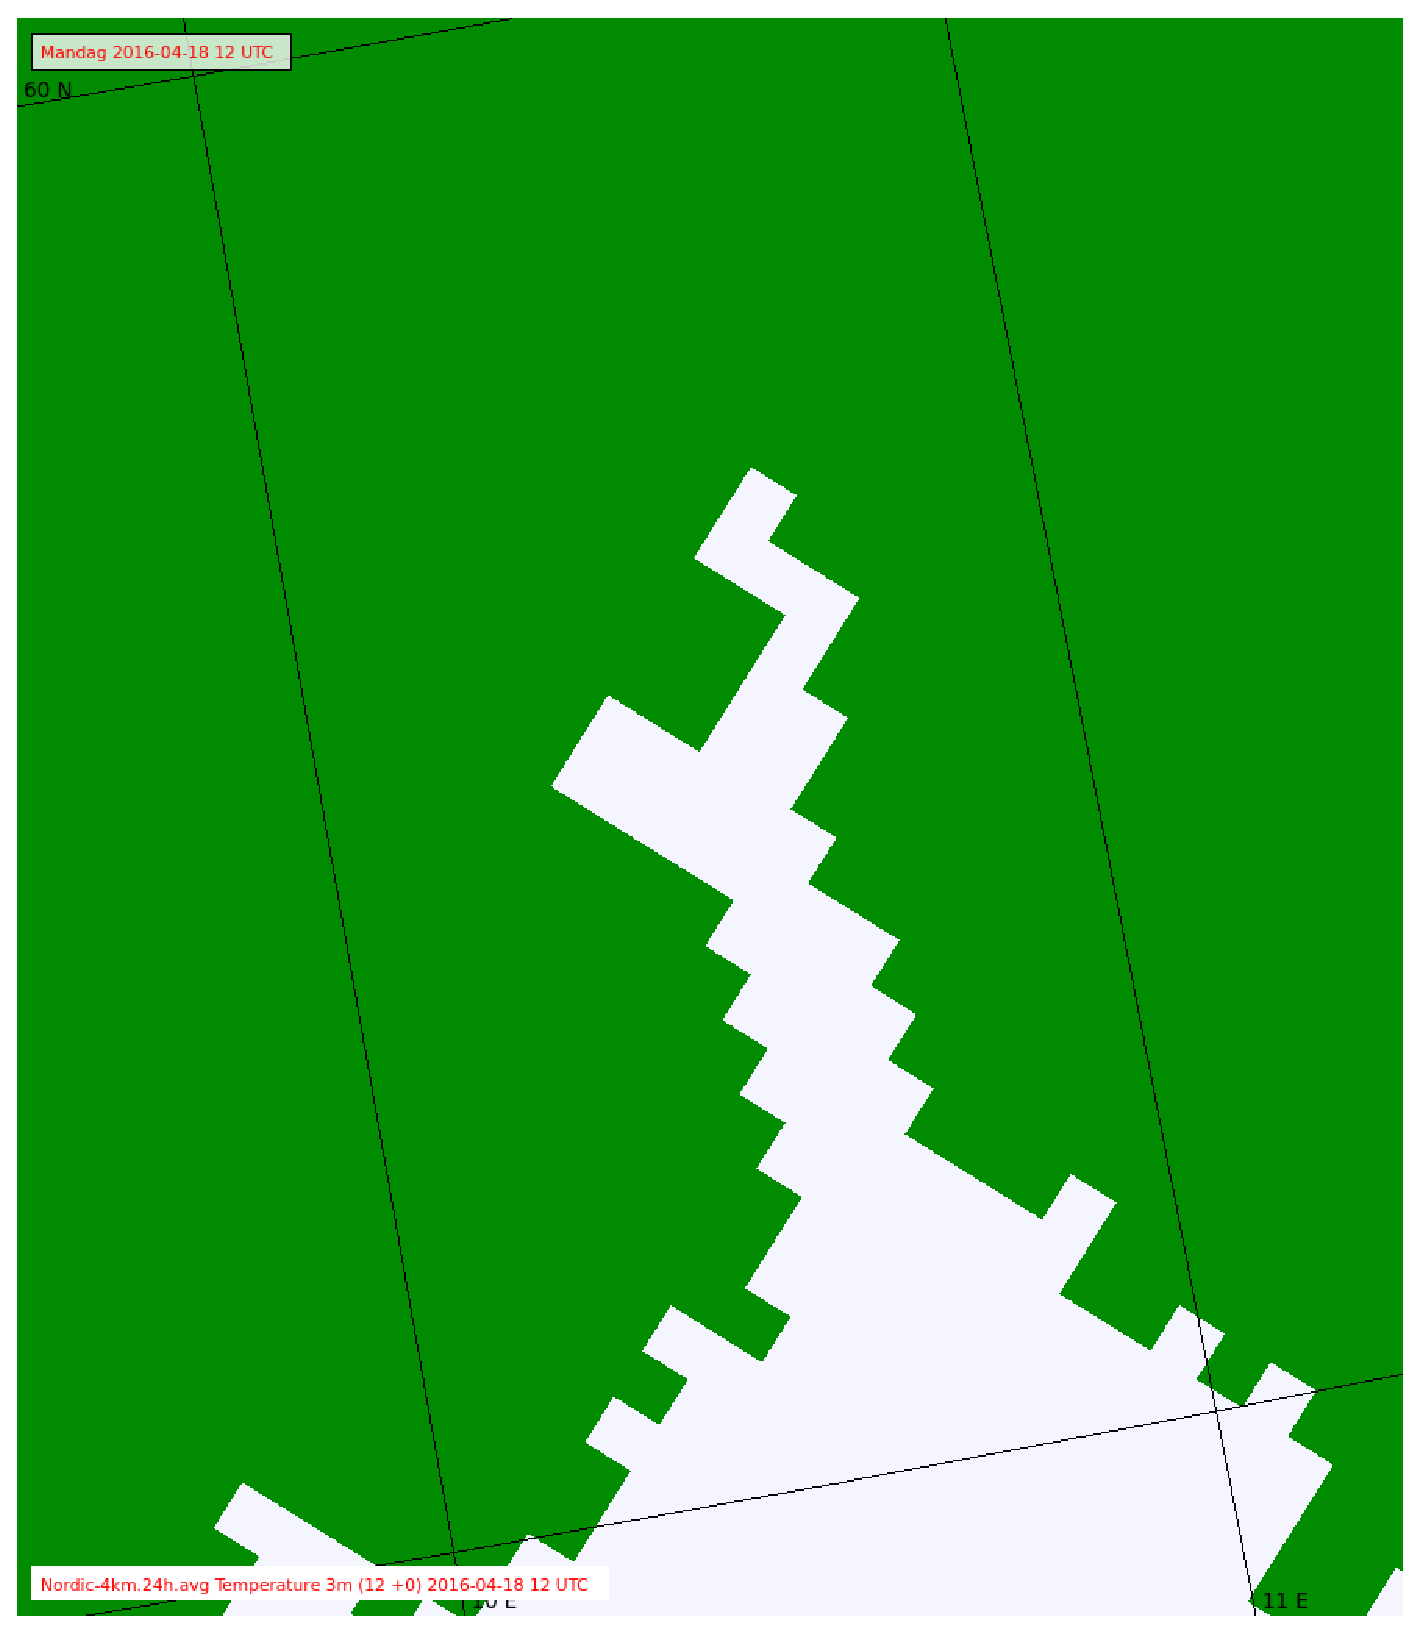
\includegraphics[height=5.2cm]{Oslofjord_N4_grid}}
   \rput[br](7.4,0.0){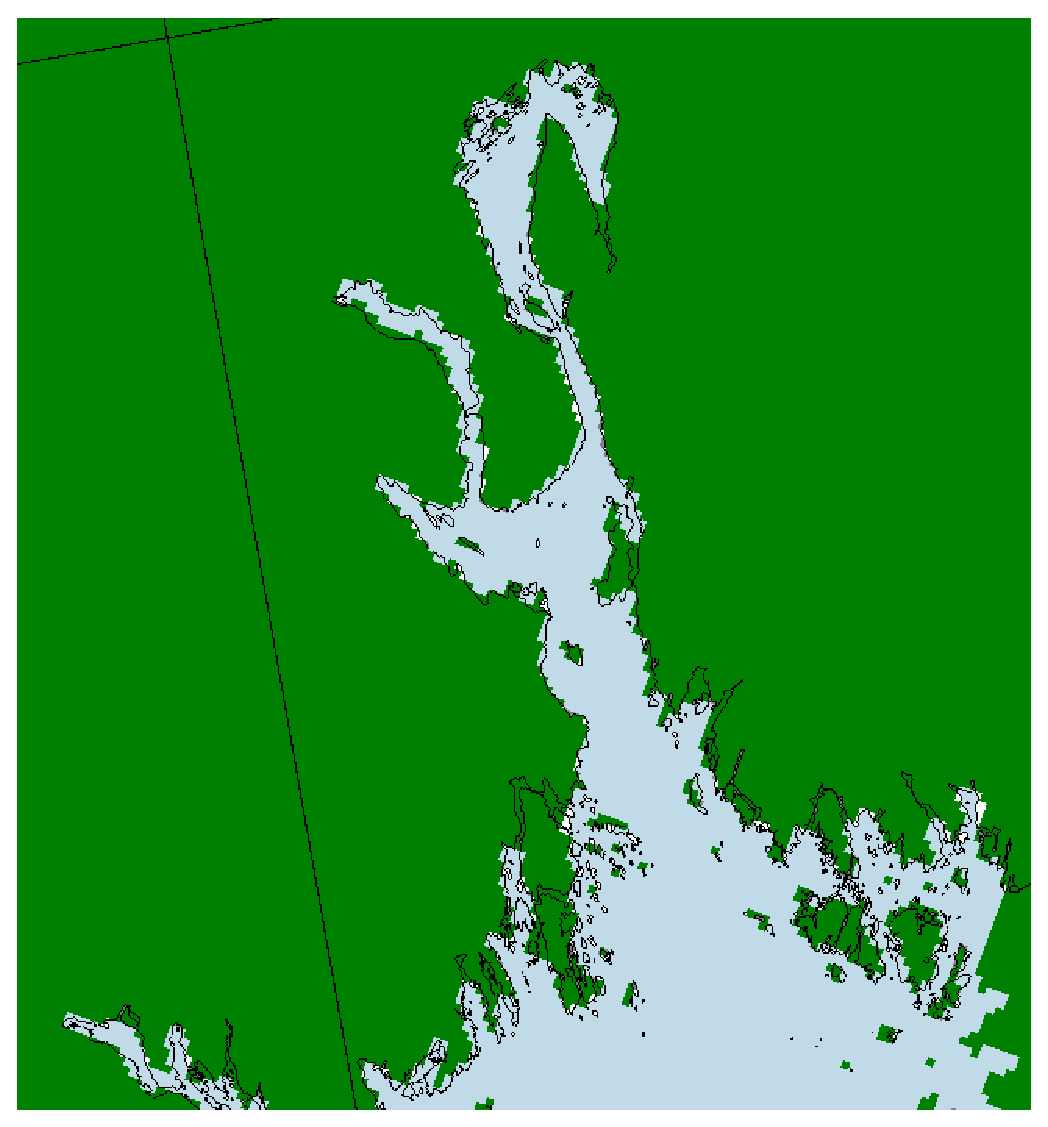
\includegraphics[height=5.2cm]{Oslofjord_N800_grid}}
   \rput[bl](7.5,0.0){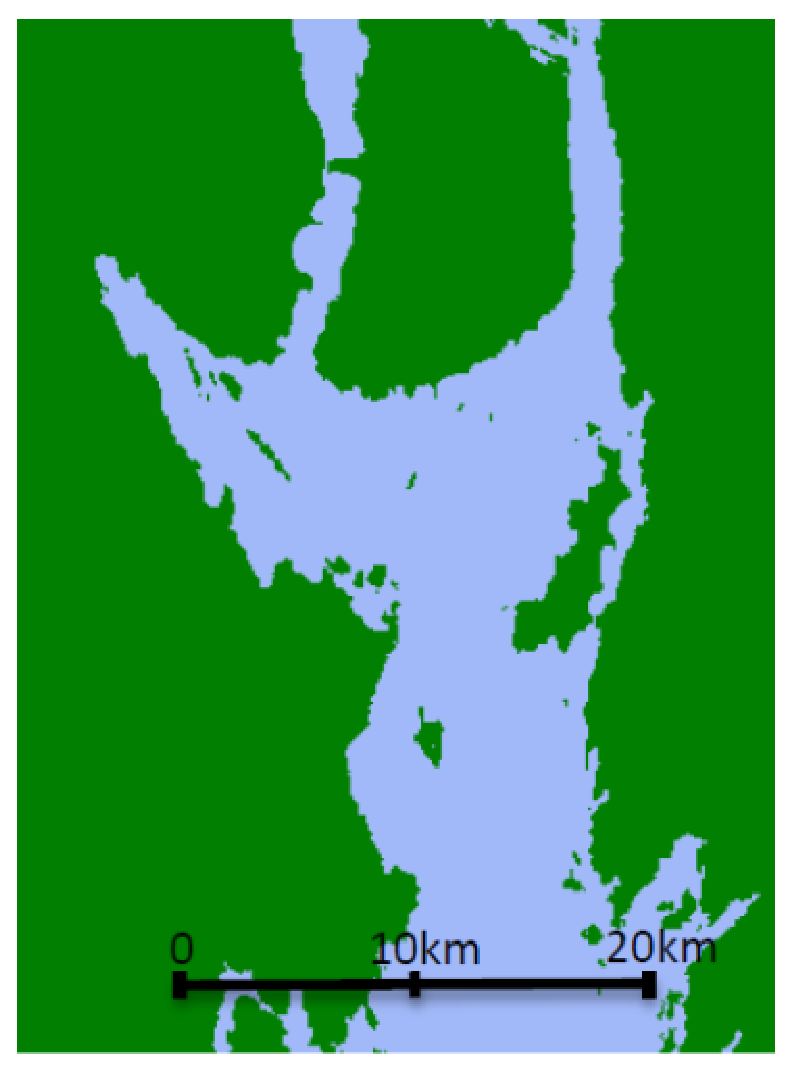
\includegraphics[height=5.2cm]{Midfjord_100m_grid}}
  \end{pspicture}
  \caption{\small Illustrated is the impact of grid resolution on how the Oslofjord is portrayed. Upper two (from left to right) show how the fjord is represented by respectively a 20 km and 4 km grid model, while the two tbottom panels show the same for respectively an 800 m and 100 m grid model zoomed in on Breidangen.} 
  \label{fig:resolution}
 \end{center}
\end{figure}

